%\begin{problem}{\textbf{\textsc{Devil's Trill}}}
%Consider a string of length $L=1\;\mathrm{m}$ and linear mass density $\lambda$\ =\ 1\ g/m, fixed on both ends and vibrating in the first normal mode with amplitude $A = 0.125 \; \mathrm{cm}$. A frictionless, negligibly-small finger, initially at the right endpoint, slides slowly toward the left, flattening the oscillation as it goes. When the vibrating part of the string has length $L_2=12.5\;\mathrm{cm}$, find the new amplitude of vibrations $A_2$, in meters. You may assume $A_2\ll L_2$. Diagrams are not necessarily drawn to scale. 

%\FloatBarrier
%\begin{figure*}[!htbp]
%\centering
%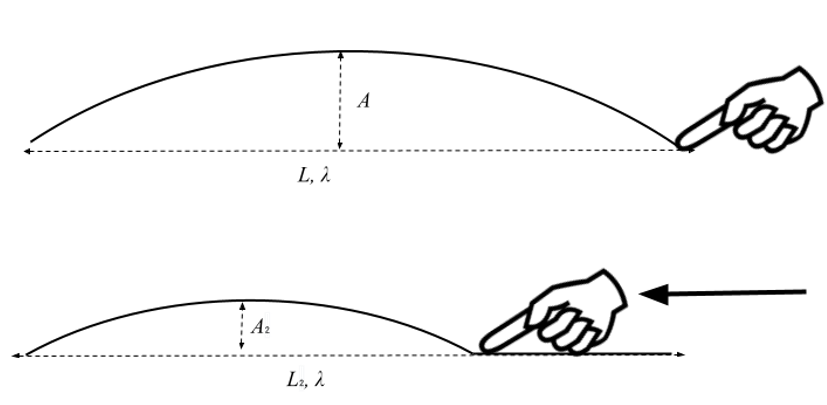
\includegraphics[width=0.6\textwidth]{problems/figures/devilTrill.png}
%\end{figure*}
%\FloatBarrier



%\end{problem}

\begin{problem}{\textbf{\textsc{Devil's Trill}}}
	Xem xét một sợi dây có chiều dài $L=1\;\mathrm{m}$ và mật độ khối lượng tuyến tính $\lambda$\ =\ 1\ g/m, được cố định ở cả hai đầu và dao động ở chế độ dao động chuẩn thứ nhất với biên độ $A = 0.125 \; \mathrm{cm}$. Một ngón tay không ma sát, có kích thước không đáng kể, ban đầu ở điểm cuối bên phải, trượt chậm về phía bên trái, làm phẳng dao động khi nó di chuyển. Khi phần dao động của sợi dây có chiều dài $L_2=12.5\;\mathrm{cm}$, hãy tìm biên độ dao động mới $A_2$, ở đơn vị mét. Bạn có thể giả sử rằng $A_2\ll L_2$. Các hình vẽ không nhất thiết phải được vẽ theo tỷ lệ. 
	
	\FloatBarrier
	\begin{figure*}[!htbp]
		\centering
		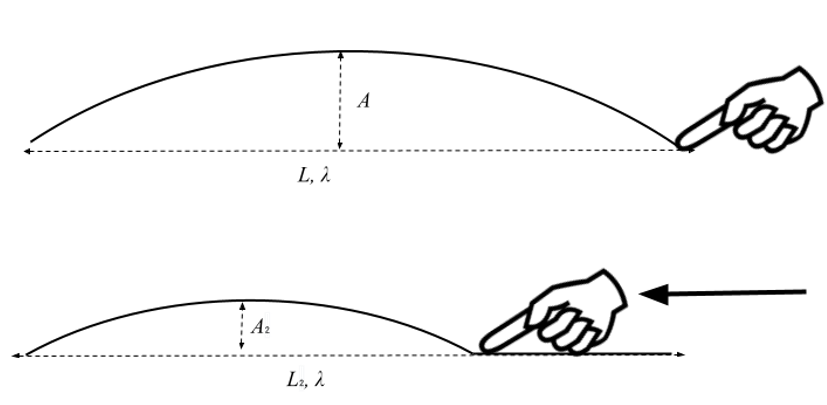
\includegraphics[width=0.6\textwidth]{problems/figures/devilTrill.png}
	\end{figure*}
	\FloatBarrier
	
	
	
\end{problem}